\documentclass[]{article}
\usepackage{lmodern}
\usepackage{amssymb,amsmath}
\usepackage{ifxetex,ifluatex}
\usepackage{fixltx2e} % provides \textsubscript
\ifnum 0\ifxetex 1\fi\ifluatex 1\fi=0 % if pdftex
  \usepackage[T1]{fontenc}
  \usepackage[utf8]{inputenc}
\else % if luatex or xelatex
  \ifxetex
    \usepackage{mathspec}
  \else
    \usepackage{fontspec}
  \fi
  \defaultfontfeatures{Ligatures=TeX,Scale=MatchLowercase}
\fi
% use upquote if available, for straight quotes in verbatim environments
\IfFileExists{upquote.sty}{\usepackage{upquote}}{}
% use microtype if available
\IfFileExists{microtype.sty}{%
\usepackage{microtype}
\UseMicrotypeSet[protrusion]{basicmath} % disable protrusion for tt fonts
}{}
\usepackage[margin=1in]{geometry}
\usepackage{hyperref}
\hypersetup{unicode=true,
            pdfauthor={Laura Biggins},
            pdfborder={0 0 0},
            breaklinks=true}
\urlstyle{same}  % don't use monospace font for urls
\usepackage{color}
\usepackage{fancyvrb}
\newcommand{\VerbBar}{|}
\newcommand{\VERB}{\Verb[commandchars=\\\{\}]}
\DefineVerbatimEnvironment{Highlighting}{Verbatim}{commandchars=\\\{\}}
% Add ',fontsize=\small' for more characters per line
\usepackage{framed}
\definecolor{shadecolor}{RGB}{248,248,248}
\newenvironment{Shaded}{\begin{snugshade}}{\end{snugshade}}
\newcommand{\KeywordTok}[1]{\textcolor[rgb]{0.13,0.29,0.53}{\textbf{#1}}}
\newcommand{\DataTypeTok}[1]{\textcolor[rgb]{0.13,0.29,0.53}{#1}}
\newcommand{\DecValTok}[1]{\textcolor[rgb]{0.00,0.00,0.81}{#1}}
\newcommand{\BaseNTok}[1]{\textcolor[rgb]{0.00,0.00,0.81}{#1}}
\newcommand{\FloatTok}[1]{\textcolor[rgb]{0.00,0.00,0.81}{#1}}
\newcommand{\ConstantTok}[1]{\textcolor[rgb]{0.00,0.00,0.00}{#1}}
\newcommand{\CharTok}[1]{\textcolor[rgb]{0.31,0.60,0.02}{#1}}
\newcommand{\SpecialCharTok}[1]{\textcolor[rgb]{0.00,0.00,0.00}{#1}}
\newcommand{\StringTok}[1]{\textcolor[rgb]{0.31,0.60,0.02}{#1}}
\newcommand{\VerbatimStringTok}[1]{\textcolor[rgb]{0.31,0.60,0.02}{#1}}
\newcommand{\SpecialStringTok}[1]{\textcolor[rgb]{0.31,0.60,0.02}{#1}}
\newcommand{\ImportTok}[1]{#1}
\newcommand{\CommentTok}[1]{\textcolor[rgb]{0.56,0.35,0.01}{\textit{#1}}}
\newcommand{\DocumentationTok}[1]{\textcolor[rgb]{0.56,0.35,0.01}{\textbf{\textit{#1}}}}
\newcommand{\AnnotationTok}[1]{\textcolor[rgb]{0.56,0.35,0.01}{\textbf{\textit{#1}}}}
\newcommand{\CommentVarTok}[1]{\textcolor[rgb]{0.56,0.35,0.01}{\textbf{\textit{#1}}}}
\newcommand{\OtherTok}[1]{\textcolor[rgb]{0.56,0.35,0.01}{#1}}
\newcommand{\FunctionTok}[1]{\textcolor[rgb]{0.00,0.00,0.00}{#1}}
\newcommand{\VariableTok}[1]{\textcolor[rgb]{0.00,0.00,0.00}{#1}}
\newcommand{\ControlFlowTok}[1]{\textcolor[rgb]{0.13,0.29,0.53}{\textbf{#1}}}
\newcommand{\OperatorTok}[1]{\textcolor[rgb]{0.81,0.36,0.00}{\textbf{#1}}}
\newcommand{\BuiltInTok}[1]{#1}
\newcommand{\ExtensionTok}[1]{#1}
\newcommand{\PreprocessorTok}[1]{\textcolor[rgb]{0.56,0.35,0.01}{\textit{#1}}}
\newcommand{\AttributeTok}[1]{\textcolor[rgb]{0.77,0.63,0.00}{#1}}
\newcommand{\RegionMarkerTok}[1]{#1}
\newcommand{\InformationTok}[1]{\textcolor[rgb]{0.56,0.35,0.01}{\textbf{\textit{#1}}}}
\newcommand{\WarningTok}[1]{\textcolor[rgb]{0.56,0.35,0.01}{\textbf{\textit{#1}}}}
\newcommand{\AlertTok}[1]{\textcolor[rgb]{0.94,0.16,0.16}{#1}}
\newcommand{\ErrorTok}[1]{\textcolor[rgb]{0.64,0.00,0.00}{\textbf{#1}}}
\newcommand{\NormalTok}[1]{#1}
\usepackage{graphicx,grffile}
\makeatletter
\def\maxwidth{\ifdim\Gin@nat@width>\linewidth\linewidth\else\Gin@nat@width\fi}
\def\maxheight{\ifdim\Gin@nat@height>\textheight\textheight\else\Gin@nat@height\fi}
\makeatother
% Scale images if necessary, so that they will not overflow the page
% margins by default, and it is still possible to overwrite the defaults
% using explicit options in \includegraphics[width, height, ...]{}
\setkeys{Gin}{width=\maxwidth,height=\maxheight,keepaspectratio}
\IfFileExists{parskip.sty}{%
\usepackage{parskip}
}{% else
\setlength{\parindent}{0pt}
\setlength{\parskip}{6pt plus 2pt minus 1pt}
}
\setlength{\emergencystretch}{3em}  % prevent overfull lines
\providecommand{\tightlist}{%
  \setlength{\itemsep}{0pt}\setlength{\parskip}{0pt}}
\setcounter{secnumdepth}{0}
% Redefines (sub)paragraphs to behave more like sections
\ifx\paragraph\undefined\else
\let\oldparagraph\paragraph
\renewcommand{\paragraph}[1]{\oldparagraph{#1}\mbox{}}
\fi
\ifx\subparagraph\undefined\else
\let\oldsubparagraph\subparagraph
\renewcommand{\subparagraph}[1]{\oldsubparagraph{#1}\mbox{}}
\fi

%%% Use protect on footnotes to avoid problems with footnotes in titles
\let\rmarkdownfootnote\footnote%
\def\footnote{\protect\rmarkdownfootnote}

%%% Change title format to be more compact
\usepackage{titling}

% Create subtitle command for use in maketitle
\newcommand{\subtitle}[1]{
  \posttitle{
    \begin{center}\large#1\end{center}
    }
}

\setlength{\droptitle}{-2em}

  \title{\begin{enumerate}
\def\labelenumi{\arabic{enumi}.}
\tightlist
\item
  Length biased gene sets
\end{enumerate}}
    \pretitle{\vspace{\droptitle}\centering\huge}
  \posttitle{\par}
    \author{Laura Biggins}
    \preauthor{\centering\large\emph}
  \postauthor{\par}
      \predate{\centering\large\emph}
  \postdate{\par}
    \date{4 March 2019}


\begin{document}
\maketitle

\begin{Shaded}
\begin{Highlighting}[]
\KeywordTok{library}\NormalTok{(}\StringTok{"devtools"}\NormalTok{)}
\KeywordTok{ifelse}\NormalTok{(using_laptop,}
       \KeywordTok{load_all}\NormalTok{(}\StringTok{"C:/Users/bigginsl/Desktop/temp/GOcategoryStats"}\NormalTok{),}
       \KeywordTok{load_all}\NormalTok{(}\StringTok{"M:/GOcategoryStats"}\NormalTok{)}
\NormalTok{       )}
\end{Highlighting}
\end{Shaded}

\begin{verbatim}
## [[1]]
## <environment: namespace:GOcategoryStats>
\end{verbatim}

\begin{Shaded}
\begin{Highlighting}[]
\KeywordTok{par}\NormalTok{(}\DataTypeTok{mgp =} \KeywordTok{c}\NormalTok{(}\DecValTok{2}\NormalTok{, }\FloatTok{0.5}\NormalTok{, }\DecValTok{0}\NormalTok{))}
\KeywordTok{par}\NormalTok{(}\DataTypeTok{mar =} \KeywordTok{par}\NormalTok{()}\OperatorTok{$}\NormalTok{mar }\OperatorTok{*}\StringTok{ }\FloatTok{0.7}\NormalTok{)}

\KeywordTok{library}\NormalTok{(RColorBrewer)}
\KeywordTok{palette}\NormalTok{(}\KeywordTok{brewer.pal}\NormalTok{(}\DecValTok{6}\NormalTok{, }\StringTok{"Set2"}\NormalTok{))}
\end{Highlighting}
\end{Shaded}

Generate lists of mouse genes biased by the length of the genes.

\subsubsection{Import the gene info
file}\label{import-the-gene-info-file}

The gene info file contains the lengths of all the genes in the mouse
genome. These can be plotted so that some thresholds for length
categories can be determined.

\subsubsection{Lengths of genes}\label{lengths-of-genes}

\paragraph{Plot out the length distribution for all the genes in
Mus\_musculus.GRCm38.94}\label{plot-out-the-length-distribution-for-all-the-genes-in-mus_musculus.grcm38.94}

\begin{Shaded}
\begin{Highlighting}[]
\NormalTok{x <-}\StringTok{ }\KeywordTok{ifelse}\NormalTok{(using_laptop,}
\NormalTok{       genfo <-}\StringTok{ }\KeywordTok{read.delim}\NormalTok{(}\StringTok{"C:/Users/bigginsl/Desktop/temp//biased_gene_lists/Mus_musculus.GRCm38.94_gene_info.txt"}\NormalTok{),}
\NormalTok{       genfo <-}\StringTok{ }\KeywordTok{read.delim}\NormalTok{(}\StringTok{"M:/biased_gene_lists/Mus_musculus.GRCm38.94_gene_info.txt"}\NormalTok{)}
\NormalTok{)}
\NormalTok{bg_genes <-}\StringTok{ }\KeywordTok{as.vector}\NormalTok{(}\KeywordTok{unique}\NormalTok{(genfo}\OperatorTok{$}\NormalTok{gene_name))}

\KeywordTok{plot}\NormalTok{(}\KeywordTok{density}\NormalTok{(}\KeywordTok{log2}\NormalTok{(genfo}\OperatorTok{$}\NormalTok{length)), }\DataTypeTok{lwd =} \DecValTok{2}\NormalTok{, }\DataTypeTok{main =} \StringTok{""}\NormalTok{, }\DataTypeTok{xlab =} \StringTok{"log2 gene length"}\NormalTok{)}
\end{Highlighting}
\end{Shaded}

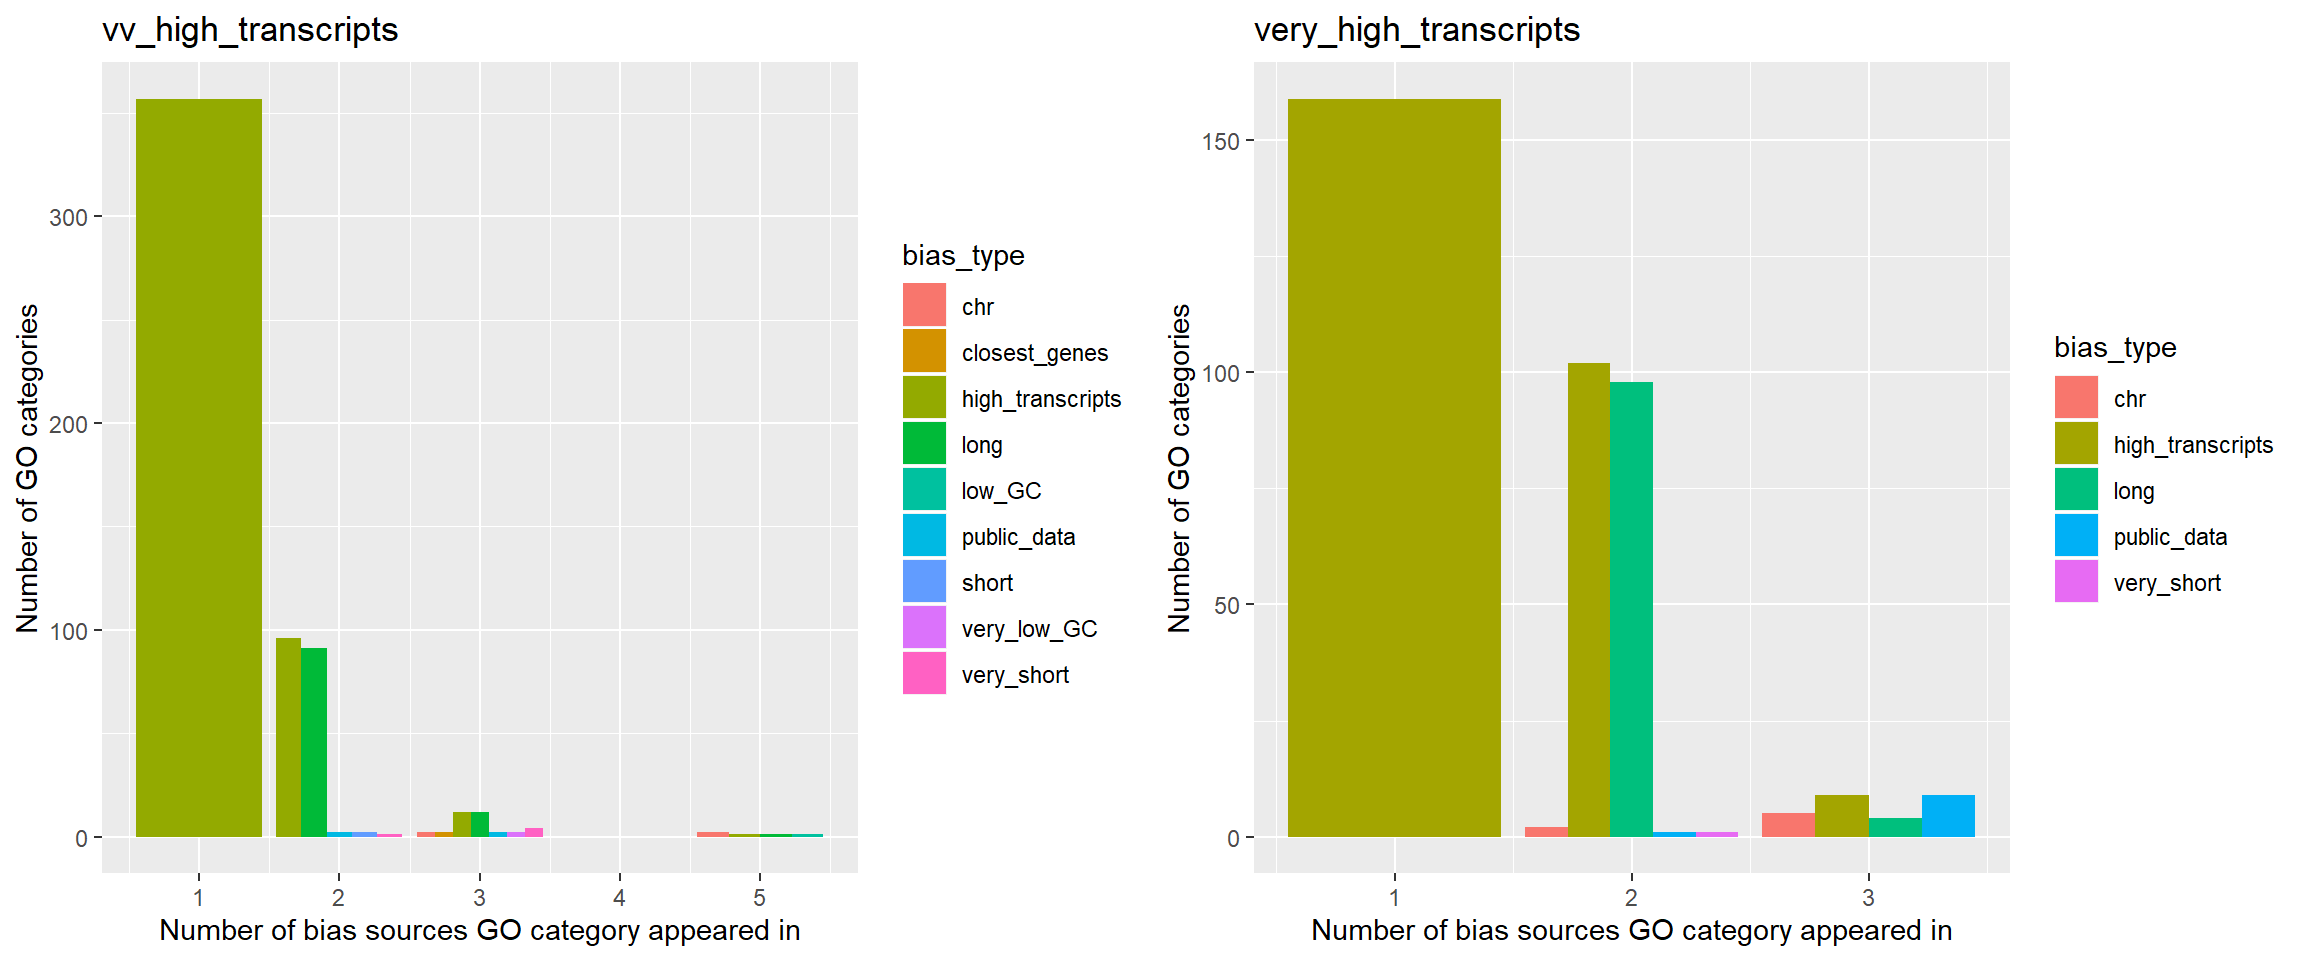
\includegraphics{1.length_biased_files/figure-latex/unnamed-chunk-4-1.pdf}

\begin{Shaded}
\begin{Highlighting}[]
\KeywordTok{boxplot}\NormalTok{(}\KeywordTok{log2}\NormalTok{(genfo}\OperatorTok{$}\NormalTok{length))}
\end{Highlighting}
\end{Shaded}

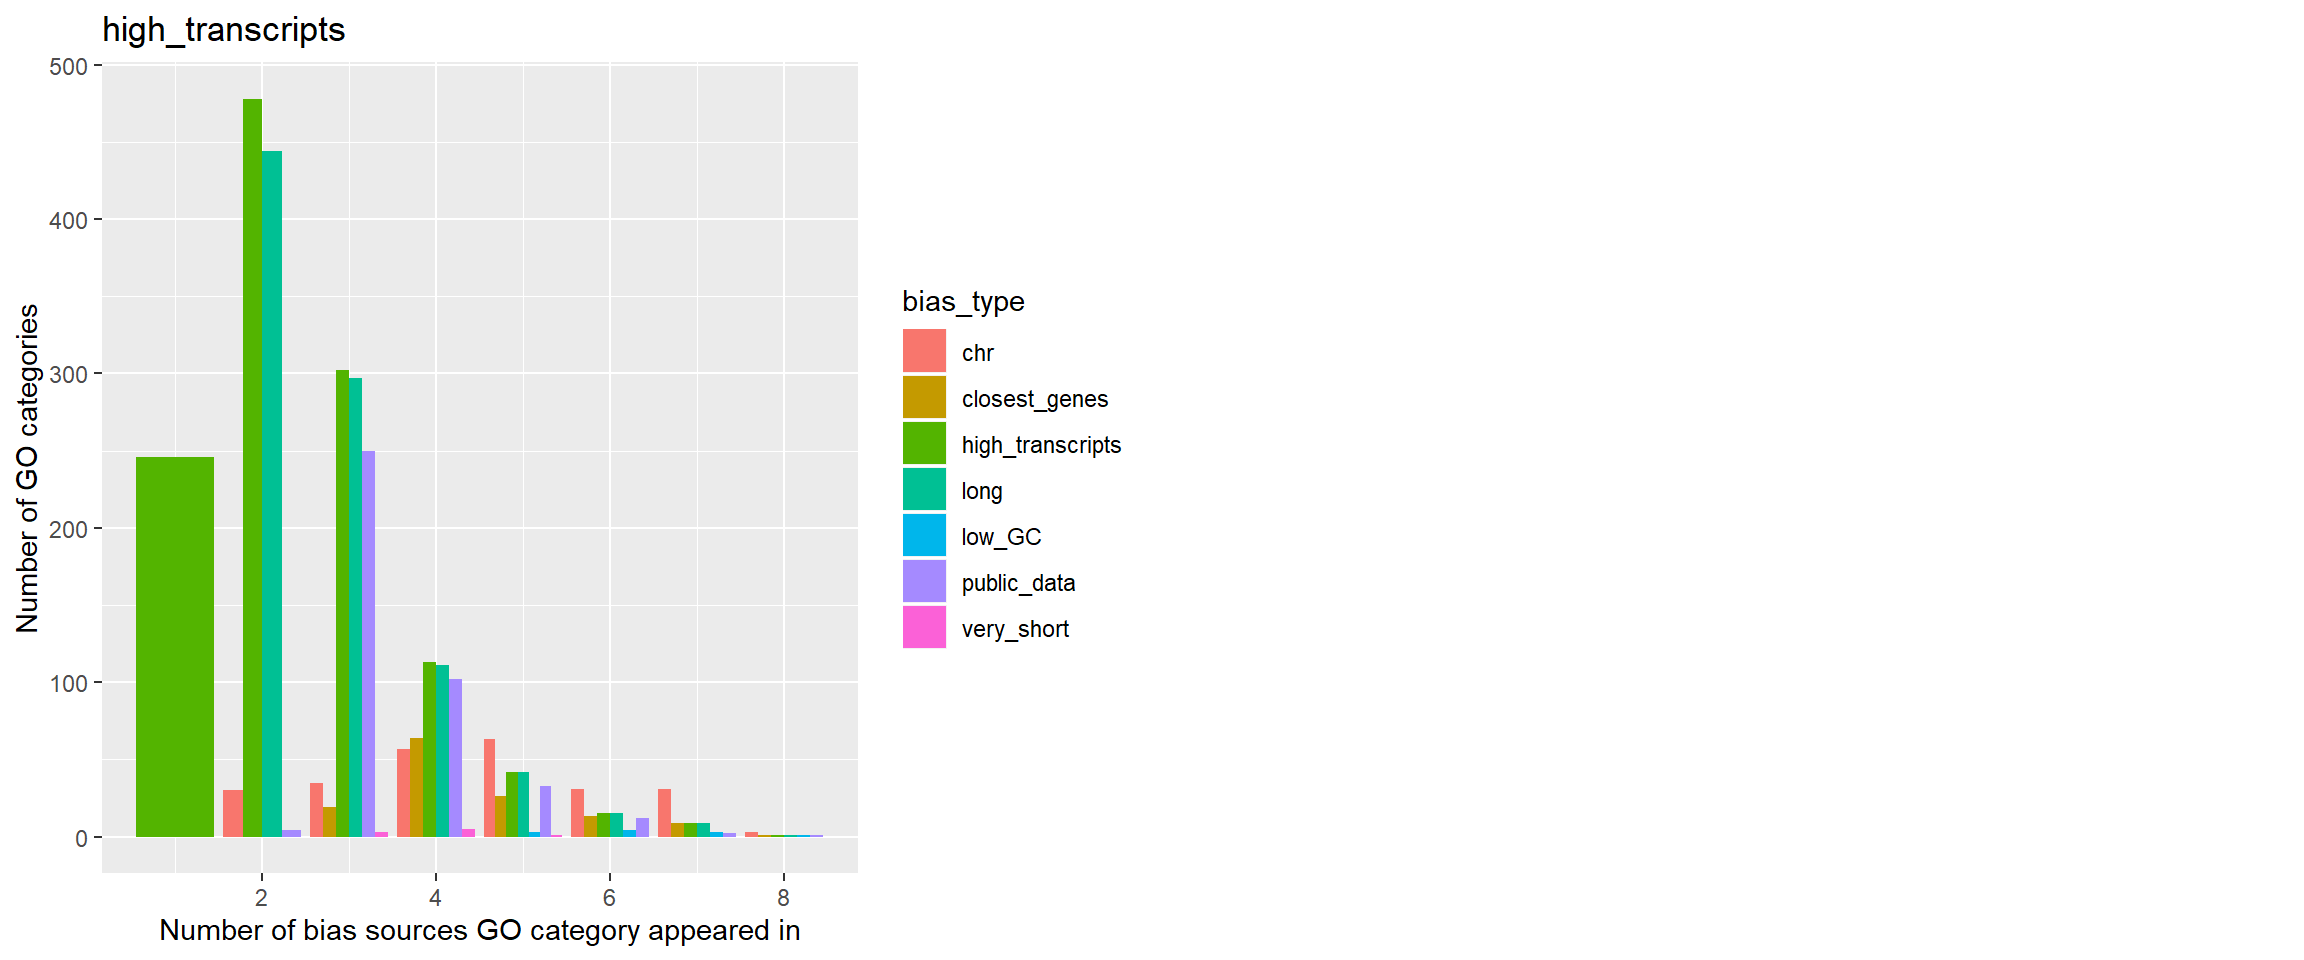
\includegraphics{1.length_biased_files/figure-latex/unnamed-chunk-4-2.pdf}

This data is displayed on a log scale as there are some very long genes
that distort the graph if it is plotted on a linear scale. The plot
shows a set of short genes between 32 and 194.0117205
(\textasciitilde{}5-7.5 on log2 scale). This provides a natural set of
lengths to use, and can be split into a ``very short'' and a ``short1''
category. We'll also take some of the genes that are slightly longer but
are below the next peak in the distribution. As the distribution of
lengths for the long genes is smooth, this provides no obvious
thresholds to select, so we can take the top 5\% and 10\% of lengths.

\begin{Shaded}
\begin{Highlighting}[]
\NormalTok{long <-}\StringTok{ }\KeywordTok{quantile}\NormalTok{(}\KeywordTok{log2}\NormalTok{(genfo}\OperatorTok{$}\NormalTok{length), }\DataTypeTok{probs =} \KeywordTok{c}\NormalTok{(}\FloatTok{0.9}\NormalTok{, }\FloatTok{0.95}\NormalTok{))}
\KeywordTok{names}\NormalTok{(long) <-}\StringTok{ }\KeywordTok{c}\NormalTok{(}\StringTok{"long"}\NormalTok{, }\StringTok{"very_long"}\NormalTok{)}
\end{Highlighting}
\end{Shaded}

\paragraph{Select gene length
thresholds.}\label{select-gene-length-thresholds.}

\begin{Shaded}
\begin{Highlighting}[]
\KeywordTok{plot}\NormalTok{(}\KeywordTok{density}\NormalTok{(}\KeywordTok{log2}\NormalTok{(genfo}\OperatorTok{$}\NormalTok{length)), }
     \DataTypeTok{lwd  =} \DecValTok{2}\NormalTok{, }
     \DataTypeTok{main =} \StringTok{""}\NormalTok{, }
     \DataTypeTok{xlab =} \StringTok{"log2 gene length"}
\NormalTok{)}

\NormalTok{thresholds <-}\StringTok{ }\KeywordTok{c}\NormalTok{(}
  \DataTypeTok{very_short =} \FloatTok{6.8}\NormalTok{, }
  \DataTypeTok{short1     =} \FloatTok{7.6}\NormalTok{, }
  \DataTypeTok{short2     =} \FloatTok{9.7}\NormalTok{, }
\NormalTok{  long}
\NormalTok{)}

\NormalTok{more_less <-}\StringTok{ }\KeywordTok{c}\NormalTok{(}
  \DataTypeTok{very_short =} \StringTok{"less"}\NormalTok{, }
  \DataTypeTok{short1     =} \StringTok{"less"}\NormalTok{, }
  \DataTypeTok{short2     =} \StringTok{"interval"}\NormalTok{, }
  \DataTypeTok{long       =} \StringTok{"more"}\NormalTok{, }
  \DataTypeTok{very_long  =} \StringTok{"more"}
\NormalTok{)}

\KeywordTok{sapply}\NormalTok{(}\KeywordTok{names}\NormalTok{(thresholds), }\ControlFlowTok{function}\NormalTok{(x)\{}
\NormalTok{  colours <-}\StringTok{ }\KeywordTok{as.factor}\NormalTok{(more_less)}
  \KeywordTok{abline}\NormalTok{(}\DataTypeTok{v =}\NormalTok{ thresholds[x], }\DataTypeTok{col =}\NormalTok{ colours[x], }\DataTypeTok{lwd =} \DecValTok{2}\NormalTok{, }\DataTypeTok{lty =} \DecValTok{2}\NormalTok{)}
\NormalTok{\})}
\end{Highlighting}
\end{Shaded}

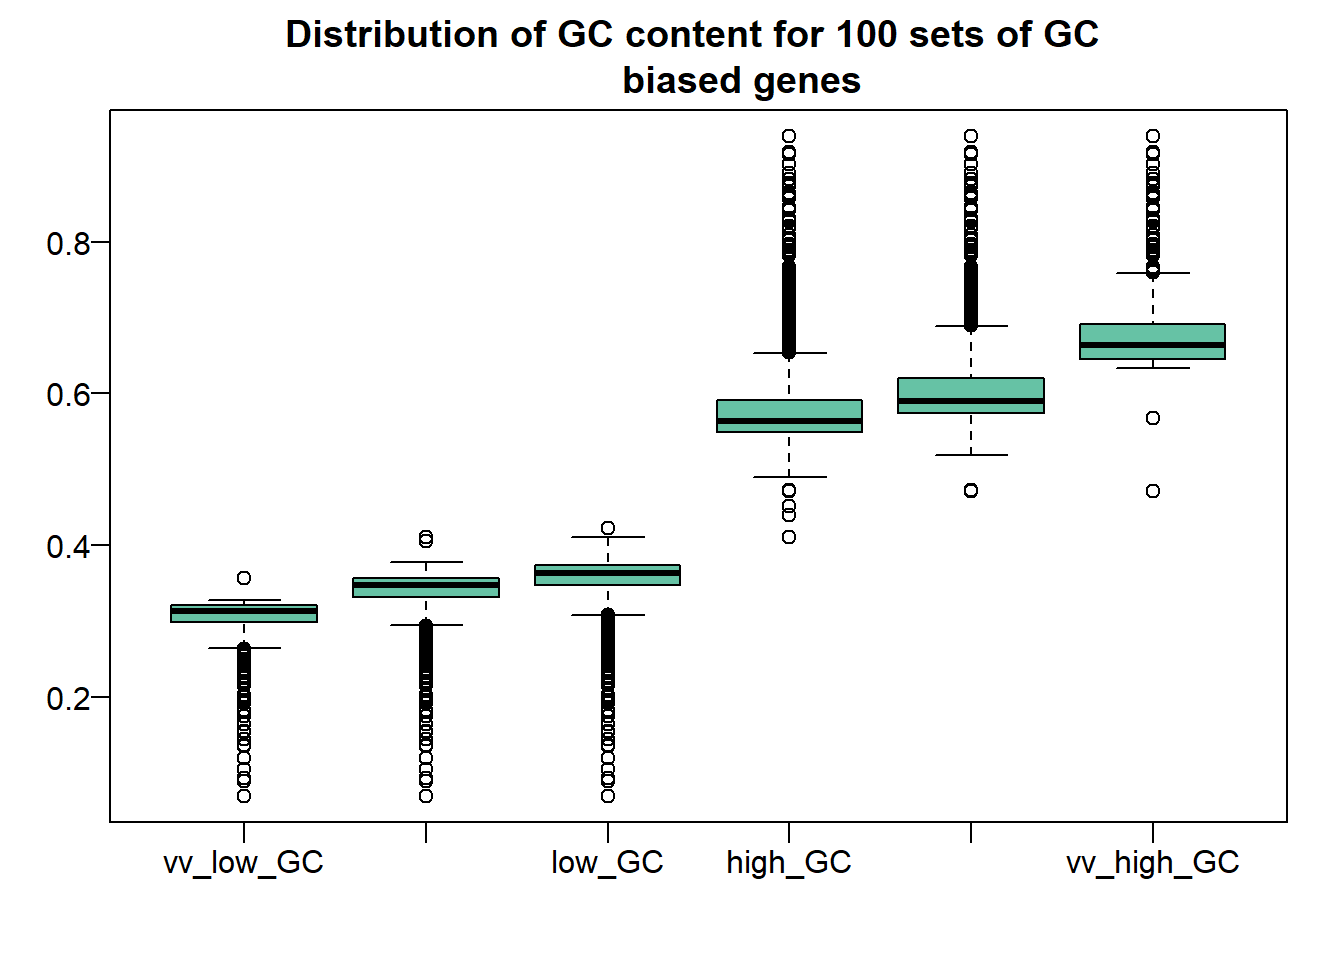
\includegraphics{1.length_biased_files/figure-latex/unnamed-chunk-6-1.pdf}

The thresholds

\begin{Shaded}
\begin{Highlighting}[]
\NormalTok{thresholds}
\end{Highlighting}
\end{Shaded}

\begin{verbatim}
## very_short     short1     short2       long  very_long 
##    6.80000    7.60000    9.70000   15.75344   16.66262
\end{verbatim}

The number of genes that remain after filtering for each length
category.

\begin{Shaded}
\begin{Highlighting}[]
\NormalTok{dens <-}\StringTok{ }\KeywordTok{density}\NormalTok{(}\KeywordTok{log2}\NormalTok{(genfo}\OperatorTok{$}\NormalTok{length))}

\KeywordTok{par}\NormalTok{(}\DataTypeTok{mfrow =} \KeywordTok{c}\NormalTok{(}\DecValTok{2}\NormalTok{, }\DecValTok{3}\NormalTok{))}

\KeywordTok{sapply}\NormalTok{(}\KeywordTok{names}\NormalTok{(thresholds), }\ControlFlowTok{function}\NormalTok{(length_cat)\{}

  \KeywordTok{plot}\NormalTok{(dens, }\DataTypeTok{lwd =} \DecValTok{2}\NormalTok{, }\DataTypeTok{xlab =} \StringTok{"log2 gene length"}\NormalTok{, }\DataTypeTok{main =}\NormalTok{ length_cat)}
  
  \ControlFlowTok{if}\NormalTok{ (more_less[length_cat] }\OperatorTok{==}\StringTok{ "less"}\NormalTok{) \{}
\NormalTok{    filt <-}\StringTok{ }\NormalTok{dens}\OperatorTok{$}\NormalTok{x }\OperatorTok{<}\StringTok{ }\NormalTok{thresholds[length_cat]}
    \KeywordTok{polygon}\NormalTok{(}
      \KeywordTok{c}\NormalTok{(dens}\OperatorTok{$}\NormalTok{x[filt], thresholds[length_cat]), }
      \KeywordTok{c}\NormalTok{(dens}\OperatorTok{$}\NormalTok{y[filt], }\DecValTok{0}\NormalTok{), }
      \DataTypeTok{col =} \StringTok{"grey"}
\NormalTok{    )}
\NormalTok{    n_genes <-}\StringTok{ }\KeywordTok{sum}\NormalTok{(}\KeywordTok{log2}\NormalTok{(genfo}\OperatorTok{$}\NormalTok{length) }\OperatorTok{<}\StringTok{ }\NormalTok{thresholds[length_cat])}
   
\NormalTok{  \} }\ControlFlowTok{else} \ControlFlowTok{if}\NormalTok{ (more_less[length_cat] }\OperatorTok{==}\StringTok{ "more"}\NormalTok{) \{}
\NormalTok{    filt <-}\StringTok{ }\NormalTok{dens}\OperatorTok{$}\NormalTok{x }\OperatorTok{>}\StringTok{ }\NormalTok{thresholds[length_cat]}
    \KeywordTok{polygon}\NormalTok{(}
      \KeywordTok{c}\NormalTok{(dens}\OperatorTok{$}\NormalTok{x[filt], thresholds[length_cat]), }
      \KeywordTok{c}\NormalTok{(dens}\OperatorTok{$}\NormalTok{y[filt], }\DecValTok{0}\NormalTok{), }
      \DataTypeTok{col =} \StringTok{"grey"}
\NormalTok{    )}
\NormalTok{    n_genes <-}\StringTok{ }\KeywordTok{sum}\NormalTok{(}\KeywordTok{log2}\NormalTok{(genfo}\OperatorTok{$}\NormalTok{length) }\OperatorTok{>}\StringTok{ }\NormalTok{thresholds[length_cat])}
    
\NormalTok{  \} }\ControlFlowTok{else}\NormalTok{ \{}
    \CommentTok{# hard code the interval plot}
\NormalTok{     filt <-}\StringTok{ }\NormalTok{dens}\OperatorTok{$}\NormalTok{x }\OperatorTok{>}\StringTok{ }\NormalTok{thresholds[}\StringTok{"short1"}\NormalTok{] }\OperatorTok{&}\StringTok{ }\NormalTok{dens}\OperatorTok{$}\NormalTok{x }\OperatorTok{<}\StringTok{ }\NormalTok{thresholds[}\StringTok{"short2"}\NormalTok{]}
     \KeywordTok{polygon}\NormalTok{(}
       \KeywordTok{c}\NormalTok{(thresholds[}\StringTok{"short1"}\NormalTok{], dens}\OperatorTok{$}\NormalTok{x[filt], thresholds[}\StringTok{"short2"}\NormalTok{]), }
       \KeywordTok{c}\NormalTok{(}\DecValTok{0}\NormalTok{, dens}\OperatorTok{$}\NormalTok{y[filt], }\DecValTok{0}\NormalTok{), }
       \DataTypeTok{col =} \StringTok{"grey"}
\NormalTok{     )}
\NormalTok{     n_genes <-}\StringTok{ }\KeywordTok{sum}\NormalTok{(}\KeywordTok{log2}\NormalTok{(genfo}\OperatorTok{$}\NormalTok{length) }\OperatorTok{>}\StringTok{ }\NormalTok{thresholds[}\StringTok{"short1"}\NormalTok{] }\OperatorTok{&}\StringTok{ }\KeywordTok{log2}\NormalTok{(genfo}\OperatorTok{$}\NormalTok{length) }\OperatorTok{<}\StringTok{ }\NormalTok{thresholds[}\StringTok{"short2"}\NormalTok{] )}
\NormalTok{  \}}
   
\NormalTok{  label_text <-}\StringTok{ }\KeywordTok{paste0}\NormalTok{(}\StringTok{"n = "}\NormalTok{, n_genes)}
  \KeywordTok{text}\NormalTok{(}\DataTypeTok{x =} \DecValTok{19}\NormalTok{, }\DataTypeTok{y =} \FloatTok{0.09}\NormalTok{, }\DataTypeTok{labels =}\NormalTok{ label_text, }\DataTypeTok{cex =} \FloatTok{1.5}\NormalTok{)}
\NormalTok{\})}
\end{Highlighting}
\end{Shaded}

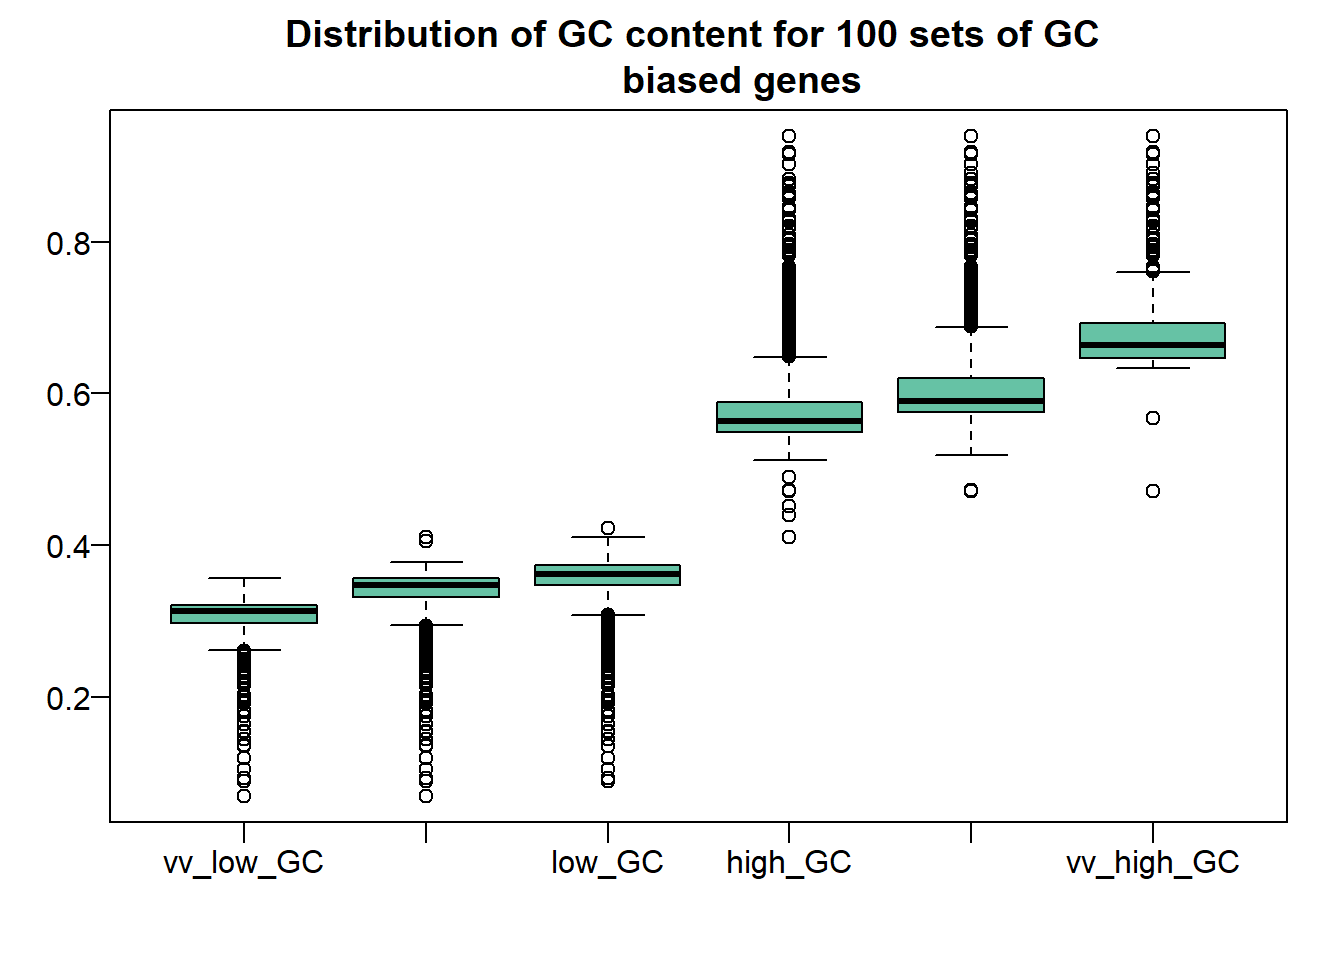
\includegraphics{1.length_biased_files/figure-latex/unnamed-chunk-8-1.pdf}

\subsubsection{Further pre-processing: Generating the biased gene
lists}\label{further-pre-processing-generating-the-biased-gene-lists}

\subsubsection{Generating the biased gene lists within
R}\label{generating-the-biased-gene-lists-within-r}

\begin{Shaded}
\begin{Highlighting}[]
\NormalTok{biased_lengths <-}\StringTok{ }\KeywordTok{lapply}\NormalTok{(}\KeywordTok{names}\NormalTok{(thresholds), }\ControlFlowTok{function}\NormalTok{(category)\{}

  \ControlFlowTok{if}\NormalTok{ (more_less[category] }\OperatorTok{==}\StringTok{ "less"}\NormalTok{) \{}
\NormalTok{    filtered_genes <-}\StringTok{ }\NormalTok{genfo}\OperatorTok{$}\NormalTok{gene_name[}\KeywordTok{log2}\NormalTok{(genfo}\OperatorTok{$}\NormalTok{length) }\OperatorTok{<}\StringTok{ }\NormalTok{thresholds[category]]}
\NormalTok{  \}}
  \ControlFlowTok{else} \ControlFlowTok{if}\NormalTok{ (more_less[category] }\OperatorTok{==}\StringTok{ "more"}\NormalTok{) \{}
\NormalTok{    filtered_genes <-}\StringTok{ }\NormalTok{genfo}\OperatorTok{$}\NormalTok{gene_name[}\KeywordTok{log2}\NormalTok{(genfo}\OperatorTok{$}\NormalTok{length) }\OperatorTok{>}\StringTok{ }\NormalTok{thresholds[category]]}
\NormalTok{  \}}
  \ControlFlowTok{else}\NormalTok{ \{}
      \CommentTok{# hard code the interval plot}
\NormalTok{     filtered_genes <-}\StringTok{ }\NormalTok{genfo}\OperatorTok{$}\NormalTok{gene_name[}\KeywordTok{log2}\NormalTok{(genfo}\OperatorTok{$}\NormalTok{length) }\OperatorTok{>}\StringTok{ }\NormalTok{thresholds[}\StringTok{"short1"}\NormalTok{] }\OperatorTok{&}\StringTok{ }
\StringTok{                                         }\KeywordTok{log2}\NormalTok{(genfo}\OperatorTok{$}\NormalTok{length) }\OperatorTok{<}\StringTok{ }\NormalTok{thresholds[}\StringTok{"short2"}\NormalTok{]]}
\NormalTok{  \}}
  \KeywordTok{sapply}\NormalTok{(}\DecValTok{1}\OperatorTok{:}\DecValTok{100}\NormalTok{, }\ControlFlowTok{function}\NormalTok{(i)\{}
\NormalTok{    filtered_genes[}\KeywordTok{ceiling}\NormalTok{(}\KeywordTok{runif}\NormalTok{(}\DecValTok{200}\NormalTok{, }\DataTypeTok{min =} \DecValTok{0}\NormalTok{, }\DataTypeTok{max =} \KeywordTok{length}\NormalTok{(filtered_genes) }\OperatorTok{-}\StringTok{ }\DecValTok{1}\NormalTok{))]}
\NormalTok{  \})}
\NormalTok{\})  }

\KeywordTok{names}\NormalTok{(biased_lengths) <-}\StringTok{ }\KeywordTok{names}\NormalTok{(thresholds)}
\end{Highlighting}
\end{Shaded}

\begin{Shaded}
\begin{Highlighting}[]
\KeywordTok{save}\NormalTok{(biased_lengths, }\DataTypeTok{file =} \StringTok{"M:/temp/length/length_genelists.rda"}\NormalTok{)}
\end{Highlighting}
\end{Shaded}

Check they all look right

\begin{Shaded}
\begin{Highlighting}[]
\KeywordTok{par}\NormalTok{(}\DataTypeTok{mfrow =} \KeywordTok{c}\NormalTok{(}\DecValTok{1}\NormalTok{, }\DecValTok{1}\NormalTok{))}

\NormalTok{lengths <-}\StringTok{ }\KeywordTok{lapply}\NormalTok{(biased_lengths, }\ControlFlowTok{function}\NormalTok{(x) \{}
  \KeywordTok{log2}\NormalTok{(genfo}\OperatorTok{$}\NormalTok{length[}\KeywordTok{match}\NormalTok{(}\KeywordTok{unlist}\NormalTok{(x), genfo}\OperatorTok{$}\NormalTok{gene_name)])}
\NormalTok{\})}

\KeywordTok{boxplot}\NormalTok{(lengths, }\DataTypeTok{col =} \DecValTok{1}\NormalTok{)}
\end{Highlighting}
\end{Shaded}

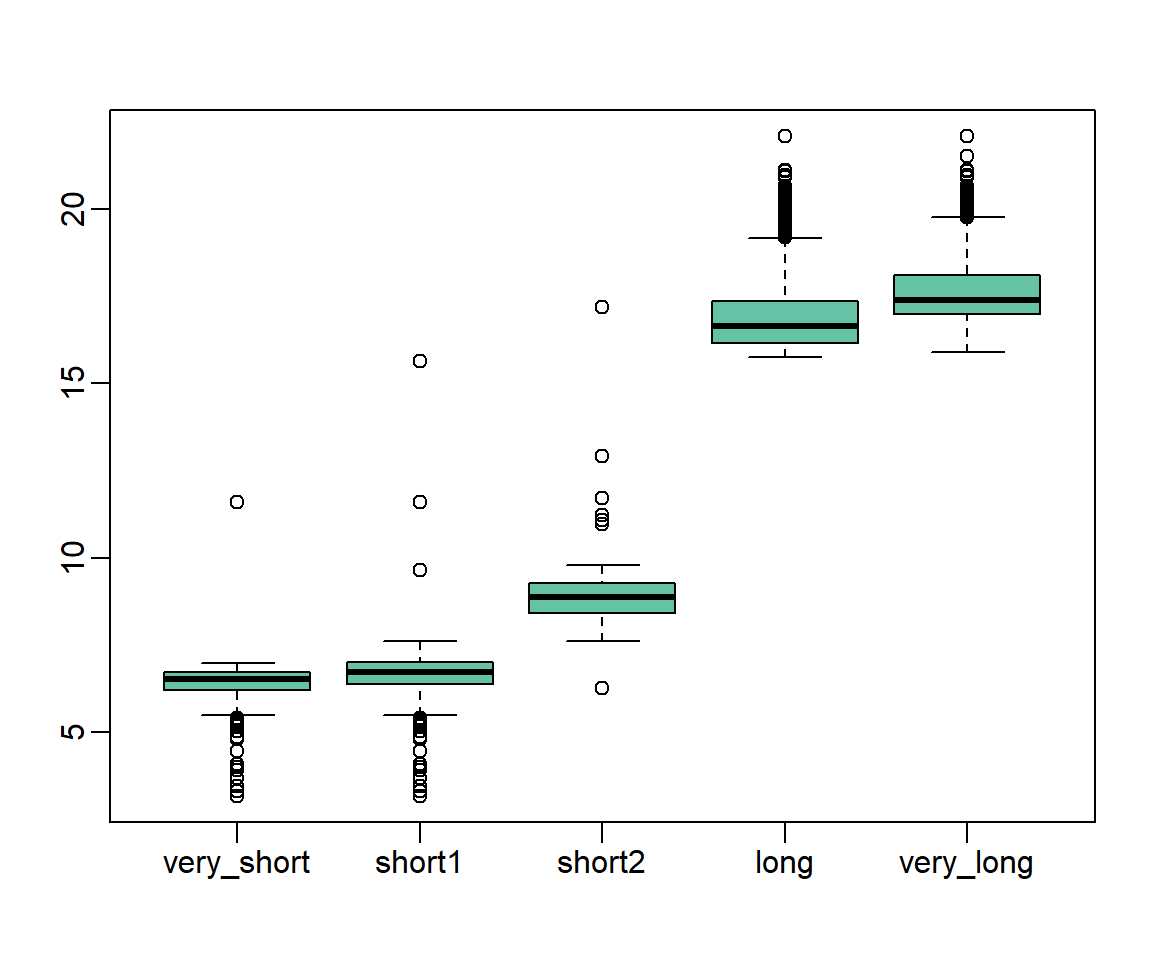
\includegraphics{1.length_biased_files/figure-latex/unnamed-chunk-10-1.pdf}

The odd gene that doesn't fall within the expected size range may be due
to name duplication.

\subsubsection{GO overrepresentation
analysis}\label{go-overrepresentation-analysis}

Run the gene lists through a GO overrepresentation analysis.

\begin{Shaded}
\begin{Highlighting}[]
\NormalTok{gene_length_results_long <-}\StringTok{ }\KeywordTok{lapply}\NormalTok{(biased_lengths[}\DecValTok{4}\OperatorTok{:}\DecValTok{5}\NormalTok{], }\ControlFlowTok{function}\NormalTok{(length_subset)\{}
  
  \KeywordTok{lapply}\NormalTok{(length_subset, }\ControlFlowTok{function}\NormalTok{(query)\{}
    \KeywordTok{overrep_test}\NormalTok{(all_go_categories, query, bg_genes)}\CommentTok{#, mult_test = FALSE)}
\NormalTok{  \})}
\NormalTok{\})}

\KeywordTok{save}\NormalTok{(gene_length_results, }\DataTypeTok{file =} \StringTok{"M:/GOcategoryStats/data/gene_length_results.rda"}\NormalTok{)}
\end{Highlighting}
\end{Shaded}

We don't want to run the GO analysis each time the document is knitted
as it takes too long. The code was run once and the data saved as an
.rda object that can be quickly loaded in to the R session.

See how many significant categories were returned.

\begin{Shaded}
\begin{Highlighting}[]
\KeywordTok{ifelse}\NormalTok{(using_laptop,}
       \KeywordTok{load}\NormalTok{(}\StringTok{"C:/Users/bigginsl/Desktop/temp//GOcategoryStats/data/length_results.rda"}\NormalTok{),}
       \KeywordTok{load}\NormalTok{(}\StringTok{"M:/GOcategoryStats/data/length_results.rda"}\NormalTok{)}
\NormalTok{)}
\end{Highlighting}
\end{Shaded}

\begin{verbatim}
## [1] "length_results"
\end{verbatim}

\begin{Shaded}
\begin{Highlighting}[]
\NormalTok{number_of_results <-}\StringTok{ }\KeywordTok{lapply}\NormalTok{(length_results, }\ControlFlowTok{function}\NormalTok{(x)\{}
\NormalTok{  nulls_removed <-}\StringTok{ }\NormalTok{x[}\KeywordTok{lapply}\NormalTok{(x,length) }\OperatorTok{!=}\StringTok{ }\DecValTok{0}\NormalTok{]}
  \KeywordTok{vapply}\NormalTok{(nulls_removed, nrow, }\DataTypeTok{FUN.VALUE =} \KeywordTok{numeric}\NormalTok{(}\DecValTok{1}\NormalTok{))}
\NormalTok{\})  }
\end{Highlighting}
\end{Shaded}

The number of gene sets that returned significant results from the GO
overrepresentation analysis

\begin{Shaded}
\begin{Highlighting}[]
\KeywordTok{sapply}\NormalTok{(number_of_results, length)}
\end{Highlighting}
\end{Shaded}

\begin{verbatim}
## very_short     short1     short2       long  very_long 
##         91         48         12        100        100
\end{verbatim}

The bean plots show the number of categories returned from each gene
list. The null results have been removed.

\begin{Shaded}
\begin{Highlighting}[]
\KeywordTok{par}\NormalTok{(}\DataTypeTok{mfrow =} \KeywordTok{c}\NormalTok{(}\DecValTok{1}\NormalTok{,}\DecValTok{1}\NormalTok{))}

\KeywordTok{library}\NormalTok{(beanplot)}
\KeywordTok{options}\NormalTok{(}\DataTypeTok{scipen =} \DecValTok{999}\NormalTok{) }\CommentTok{# disable the scientific notation}

\KeywordTok{beanplot}\NormalTok{(}
\NormalTok{  number_of_results, }
  \DataTypeTok{what   =} \KeywordTok{c}\NormalTok{(}\DecValTok{0}\NormalTok{,}\DecValTok{1}\NormalTok{,}\DecValTok{0}\NormalTok{,}\DecValTok{1}\NormalTok{), }
  \DataTypeTok{col    =} \KeywordTok{c}\NormalTok{(}\StringTok{"#1B9E77"}\NormalTok{,}\StringTok{"#06086d"}\NormalTok{), }
  \DataTypeTok{ll     =} \FloatTok{0.03}\NormalTok{, }
  \DataTypeTok{method =} \StringTok{"jitter"}\NormalTok{, }
  \DataTypeTok{border =} \StringTok{"#06086d"}\NormalTok{,}
  \DataTypeTok{las    =} \DecValTok{1}\NormalTok{,}
  \DataTypeTok{main   =} \StringTok{"number of significant categories per gene list returned from GO analysis"}
\NormalTok{)}
\end{Highlighting}
\end{Shaded}

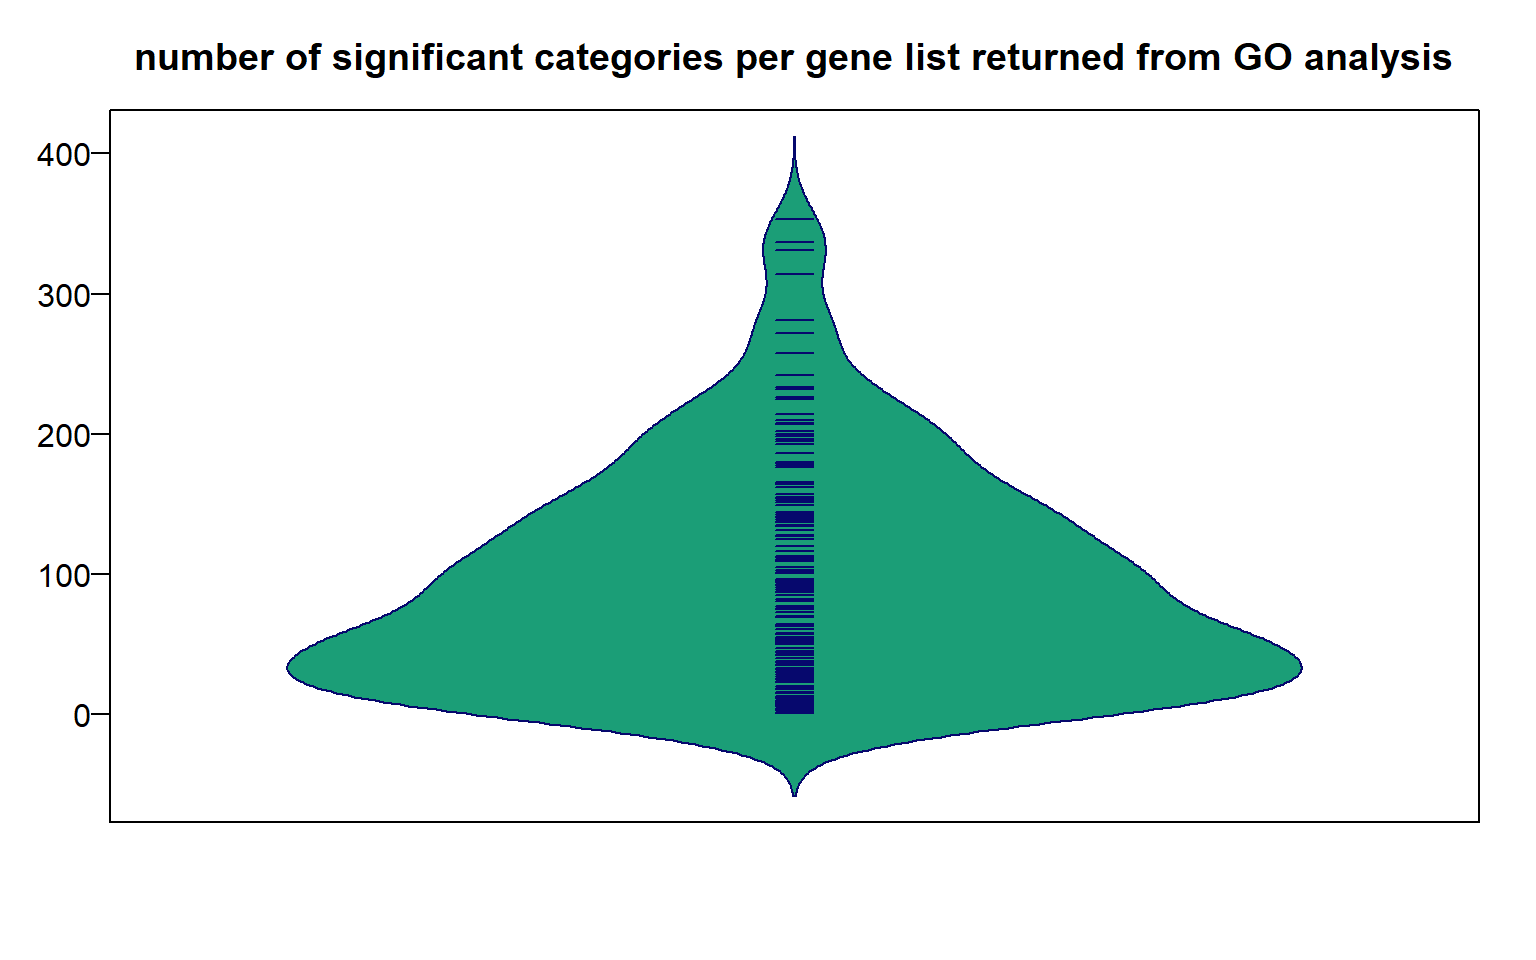
\includegraphics{1.length_biased_files/figure-latex/beanplots-1.pdf}

There are loads of results returned for the long genes, we'll plot out
the p and q values.

\begin{Shaded}
\begin{Highlighting}[]
\NormalTok{p_and_q <-}\StringTok{ }\KeywordTok{lapply}\NormalTok{(length_results, }\ControlFlowTok{function}\NormalTok{(x)\{}
\NormalTok{  pvals <-}\StringTok{ }\KeywordTok{unlist}\NormalTok{(}\KeywordTok{sapply}\NormalTok{(x, }\StringTok{`}\DataTypeTok{[[}\StringTok{`}\NormalTok{, }\StringTok{"pval"}\NormalTok{))}
\NormalTok{  qvals <-}\StringTok{ }\KeywordTok{unlist}\NormalTok{(}\KeywordTok{sapply}\NormalTok{(x, }\StringTok{`}\DataTypeTok{[[}\StringTok{`}\NormalTok{, }\StringTok{"adj_pval"}\NormalTok{))}
  \KeywordTok{data.frame}\NormalTok{(pvals, qvals)}
\NormalTok{\})}

\KeywordTok{par}\NormalTok{(}\DataTypeTok{mfrow =} \KeywordTok{c}\NormalTok{(}\KeywordTok{length}\NormalTok{(p_and_q), }\DecValTok{2}\NormalTok{))}


\NormalTok{plot_density_highlight <-}\StringTok{ }\ControlFlowTok{function}\NormalTok{(data_values, }
                                   \DataTypeTok{xlabel    =} \StringTok{""}\NormalTok{, }
                                   \DataTypeTok{threshold =} \FloatTok{0.05}\NormalTok{, }
                                   \DataTypeTok{title     =} \StringTok{""}\NormalTok{, }
                                   \DataTypeTok{colour    =} \DecValTok{3}
\NormalTok{                                   )\{}
  
\NormalTok{  dens <-}\StringTok{ }\KeywordTok{density}\NormalTok{(data_values)}
\NormalTok{  filt <-}\StringTok{ }\NormalTok{dens}\OperatorTok{$}\NormalTok{x }\OperatorTok{<}\StringTok{ }\NormalTok{threshold }
  
  \KeywordTok{plot}\NormalTok{(dens, }
    \DataTypeTok{main =}\NormalTok{ title, }
    \DataTypeTok{xlab =}\NormalTok{ xlabel,}
    \DataTypeTok{ylim =} \KeywordTok{c}\NormalTok{(}\DecValTok{0}\NormalTok{, }\KeywordTok{max}\NormalTok{(dens}\OperatorTok{$}\NormalTok{y) }\OperatorTok{*}\StringTok{ }\FloatTok{1.2}\NormalTok{) }
\NormalTok{  )}
  \KeywordTok{polygon}\NormalTok{(}
      \KeywordTok{c}\NormalTok{(dens}\OperatorTok{$}\NormalTok{x[filt], threshold), }
      \KeywordTok{c}\NormalTok{(dens}\OperatorTok{$}\NormalTok{y[filt], }\DecValTok{0}\NormalTok{), }
      \DataTypeTok{col =}\NormalTok{ colour}
\NormalTok{    )}
\NormalTok{  text_label =}\StringTok{ }\KeywordTok{paste0}\NormalTok{(}\StringTok{"n = "}\NormalTok{, }\KeywordTok{sum}\NormalTok{(data_values }\OperatorTok{<}\StringTok{ }\NormalTok{threshold))}
  \KeywordTok{text}\NormalTok{(dens}\OperatorTok{$}\NormalTok{x[}\KeywordTok{length}\NormalTok{(dens}\OperatorTok{$}\NormalTok{x)}\OperatorTok{/}\DecValTok{10}\NormalTok{], }
       \DataTypeTok{y =} \KeywordTok{max}\NormalTok{(dens}\OperatorTok{$}\NormalTok{y) }\OperatorTok{*}\StringTok{ }\FloatTok{1.1}\NormalTok{, }
       \DataTypeTok{labels =}\NormalTok{ text_label, }
       \DataTypeTok{font =} \DecValTok{2}\NormalTok{, }
       \DataTypeTok{col  =} \StringTok{"red2"}
\NormalTok{       )}
\NormalTok{\}}

\KeywordTok{sapply}\NormalTok{(}\KeywordTok{names}\NormalTok{(p_and_q), }\ControlFlowTok{function}\NormalTok{(x) \{  }
  
\NormalTok{  x_suffix <-}\StringTok{ }\KeywordTok{paste0}\NormalTok{(}\StringTok{"values, N = "}\NormalTok{, }\KeywordTok{nrow}\NormalTok{(p_and_q[[x]]))}
  
  \KeywordTok{plot_density_highlight}\NormalTok{(p_and_q[[x]]}\OperatorTok{$}\NormalTok{pvals, }
                         \DataTypeTok{title  =}\NormalTok{ x, }
                         \DataTypeTok{xlabel =} \KeywordTok{paste0}\NormalTok{(}\StringTok{"p "}\NormalTok{, x_suffix)}
\NormalTok{  )}

  \KeywordTok{plot_density_highlight}\NormalTok{(p_and_q[[x]]}\OperatorTok{$}\NormalTok{qvals, }
                         \DataTypeTok{title  =}\NormalTok{ x, }
                         \DataTypeTok{xlabel =} \KeywordTok{paste0}\NormalTok{(}\StringTok{"corrected p "}\NormalTok{, x_suffix)}
\NormalTok{  )}
\NormalTok{\})}
\end{Highlighting}
\end{Shaded}

\includegraphics{1.length_biased_files/figure-latex/p_values-1.pdf}

\begin{Shaded}
\begin{Highlighting}[]
\NormalTok{ordered_categories <-}\StringTok{ }\KeywordTok{lapply}\NormalTok{(length_results, }\ControlFlowTok{function}\NormalTok{(length_subset)\{}
  
\NormalTok{  all_sig_categories <-}\StringTok{ }\KeywordTok{unlist}\NormalTok{(}\KeywordTok{sapply}\NormalTok{(length_subset, rownames))}
\NormalTok{  tabled_categories  <-}\StringTok{ }\KeywordTok{table}\NormalTok{(all_sig_categories)}
\NormalTok{  tabled_categories[}\KeywordTok{order}\NormalTok{(tabled_categories, }\DataTypeTok{decreasing =} \OtherTok{TRUE}\NormalTok{)]}
\NormalTok{\})}

\CommentTok{#lapply(ordered_categories, head, n = 10)}
\end{Highlighting}
\end{Shaded}

Plot how many times a category appeared.

\begin{Shaded}
\begin{Highlighting}[]
\KeywordTok{par}\NormalTok{(}\DataTypeTok{mfrow =} \KeywordTok{c}\NormalTok{(}\DecValTok{2}\NormalTok{, }\DecValTok{3}\NormalTok{))}
\KeywordTok{sapply}\NormalTok{(}\KeywordTok{names}\NormalTok{(ordered_categories), }\ControlFlowTok{function}\NormalTok{(x)\{}
  \KeywordTok{plot}\NormalTok{(}\KeywordTok{density}\NormalTok{(ordered_categories[[x]]), }\DataTypeTok{main =}\NormalTok{ x)}
\NormalTok{\})}
\end{Highlighting}
\end{Shaded}

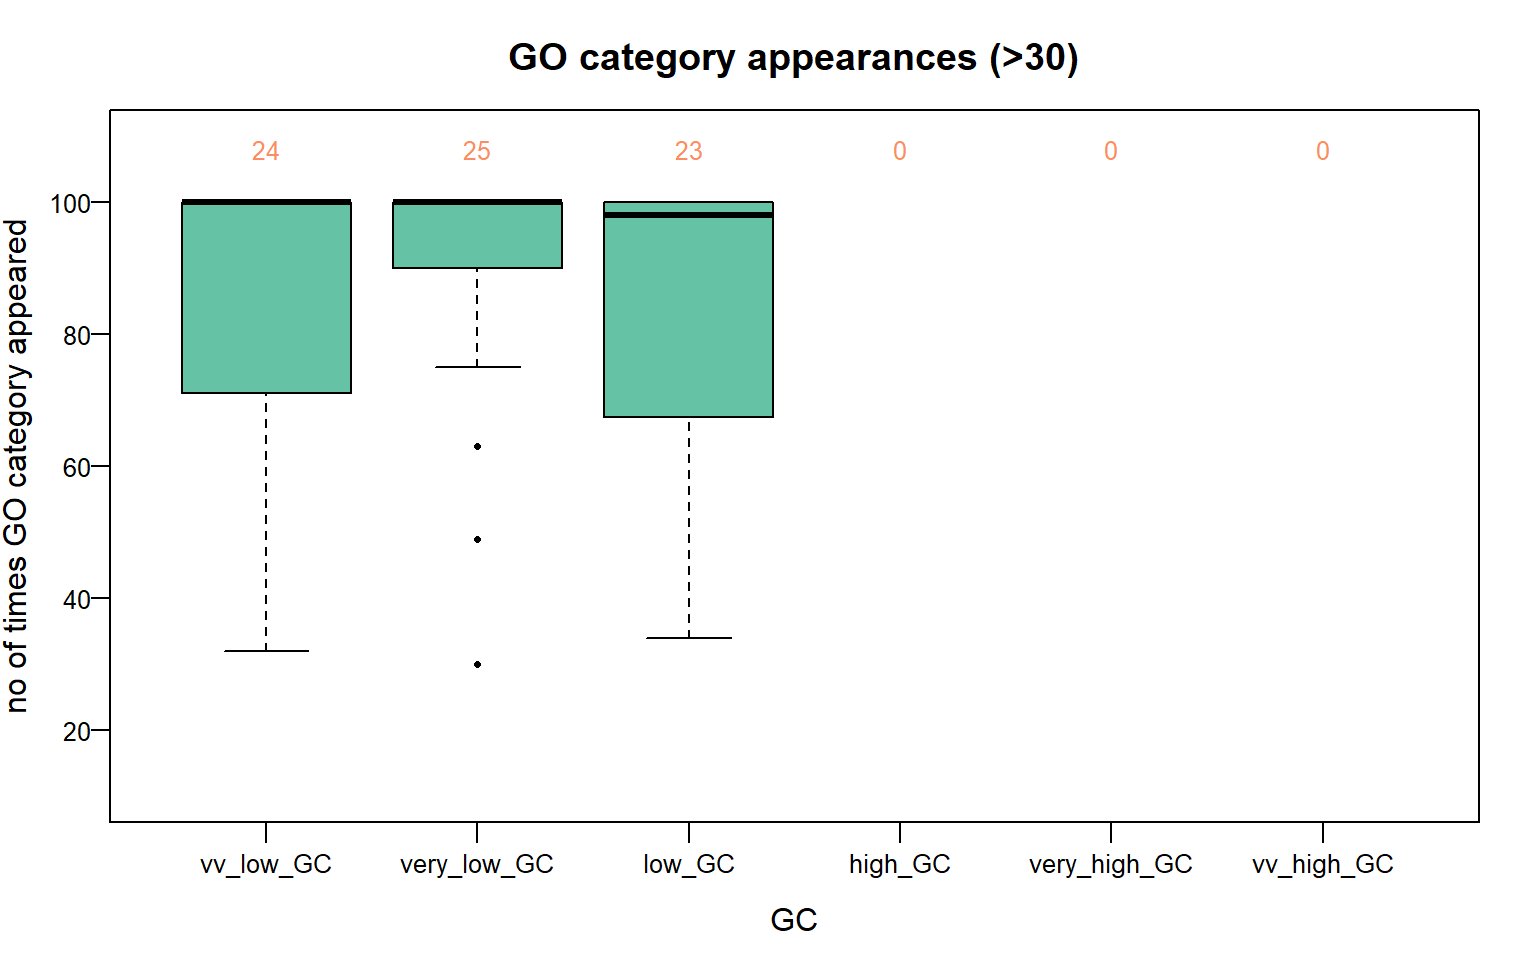
\includegraphics{1.length_biased_files/figure-latex/unnamed-chunk-14-1.pdf}

\begin{Shaded}
\begin{Highlighting}[]
\KeywordTok{par}\NormalTok{(}\DataTypeTok{mfrow =} \KeywordTok{c}\NormalTok{(}\DecValTok{1}\NormalTok{,}\DecValTok{1}\NormalTok{))}

\KeywordTok{beanplot}\NormalTok{(}
\NormalTok{  ordered_categories, }
  \DataTypeTok{what   =} \KeywordTok{c}\NormalTok{(}\DecValTok{0}\NormalTok{,}\DecValTok{1}\NormalTok{,}\DecValTok{0}\NormalTok{,}\DecValTok{1}\NormalTok{), }
  \DataTypeTok{col    =} \KeywordTok{c}\NormalTok{(}\StringTok{"#1B9E77"}\NormalTok{,}\StringTok{"#06086d"}\NormalTok{), }
  \DataTypeTok{ll     =} \FloatTok{0.03}\NormalTok{, }
  \DataTypeTok{method =} \StringTok{"jitter"}\NormalTok{, }
  \DataTypeTok{border =} \StringTok{"#06086d"}\NormalTok{,}
  \DataTypeTok{las    =} \DecValTok{1}\NormalTok{,}
  \DataTypeTok{log    =} \StringTok{""}\NormalTok{,}
  \DataTypeTok{ylim   =} \KeywordTok{c}\NormalTok{(}\DecValTok{0}\NormalTok{, }\DecValTok{120}\NormalTok{),}
  \DataTypeTok{main  =} \StringTok{"number of times a GO category appeared during the 100 tests"}\NormalTok{,}
  \DataTypeTok{ylab  =} \StringTok{"no of times GO category appeared"}
\NormalTok{)}

\KeywordTok{text}\NormalTok{(}\DecValTok{1}\OperatorTok{:}\KeywordTok{length}\NormalTok{(ordered_categories), }
     \DataTypeTok{y   =} \DecValTok{115}\NormalTok{, }
     \DataTypeTok{cex =} \FloatTok{0.8}\NormalTok{, }
     \DataTypeTok{labels =} \KeywordTok{paste0}\NormalTok{(}\StringTok{"n = "}\NormalTok{, }\KeywordTok{sapply}\NormalTok{(ordered_categories, length))}
\NormalTok{     )}
\end{Highlighting}
\end{Shaded}

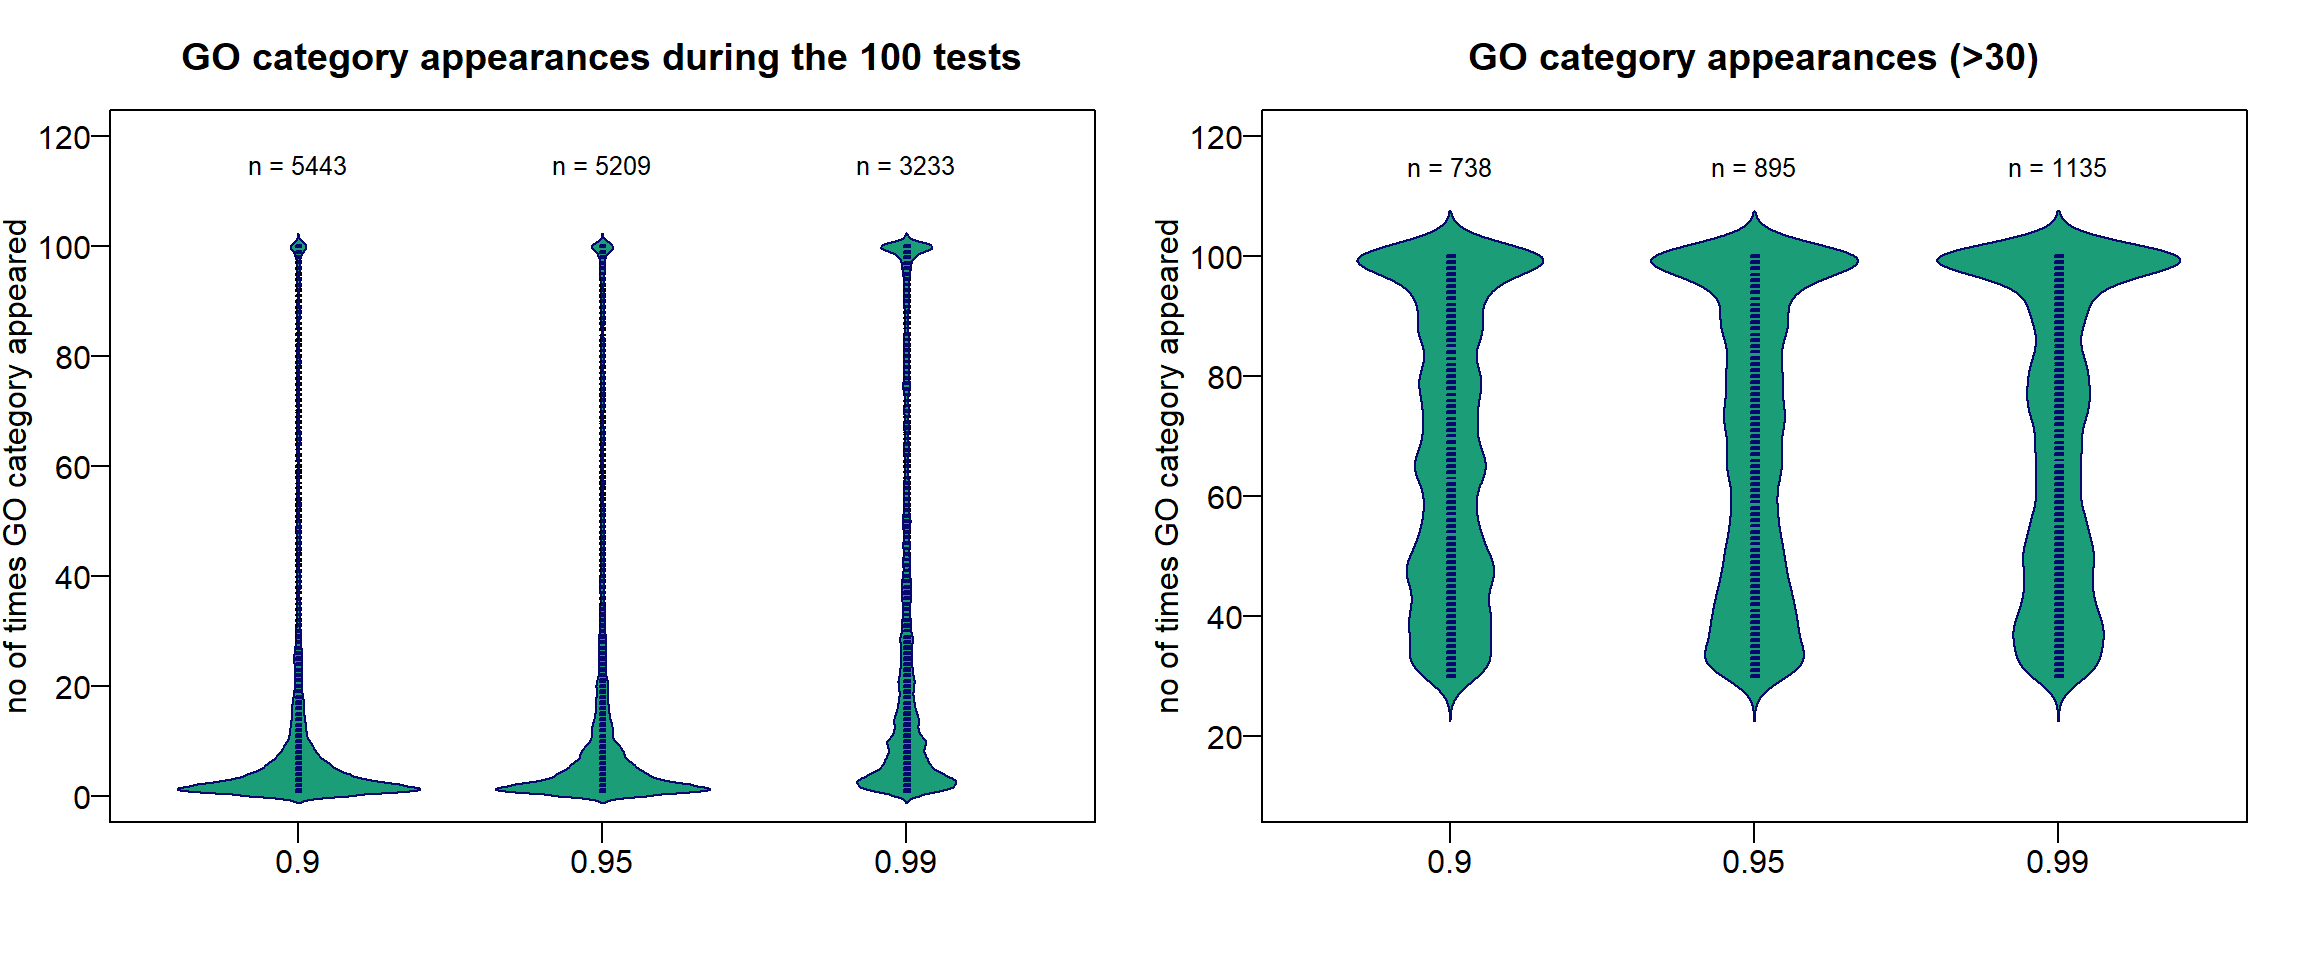
\includegraphics{1.length_biased_files/figure-latex/beanplot2-1.pdf}

\begin{Shaded}
\begin{Highlighting}[]
\NormalTok{filtered_categories <-}\StringTok{ }\KeywordTok{lapply}\NormalTok{(ordered_categories, }\ControlFlowTok{function}\NormalTok{(x) x[x }\OperatorTok{>=}\StringTok{ }\DecValTok{10}\NormalTok{])}
\end{Highlighting}
\end{Shaded}

\begin{Shaded}
\begin{Highlighting}[]
\CommentTok{# convert list of table to list of vectors}
\NormalTok{convert_tbl_vec <-}\StringTok{ }\ControlFlowTok{function}\NormalTok{(list_of_tables)\{}
\NormalTok{  list_of_vec <-}\StringTok{ }\KeywordTok{lapply}\NormalTok{(}\KeywordTok{names}\NormalTok{(list_of_tables), }\ControlFlowTok{function}\NormalTok{(x)\{}
  
\NormalTok{    vector <-}\StringTok{ }\KeywordTok{as.vector}\NormalTok{(list_of_tables[[x]])}
    \KeywordTok{names}\NormalTok{(vector) <-}\StringTok{ }\KeywordTok{names}\NormalTok{(list_of_tables[[x]])}
\NormalTok{    vector}
\NormalTok{  \})}
  \KeywordTok{names}\NormalTok{(list_of_vec) <-}\StringTok{ }\KeywordTok{names}\NormalTok{(list_of_tables)}
\NormalTok{  list_of_vec}
\NormalTok{\}}
\end{Highlighting}
\end{Shaded}

\begin{Shaded}
\begin{Highlighting}[]
\NormalTok{filtered_categories <-}\StringTok{ }\KeywordTok{lapply}\NormalTok{(ordered_categories, }\ControlFlowTok{function}\NormalTok{(x) x[x }\OperatorTok{>=}\StringTok{ }\DecValTok{10}\NormalTok{])}

\NormalTok{filtered_categories_vec <-}\StringTok{ }\KeywordTok{convert_tbl_vec}\NormalTok{(filtered_categories) }

\KeywordTok{boxplot}\NormalTok{(filtered_categories_vec,}
        \DataTypeTok{main =} \StringTok{"GO category appearances (>10)"}\NormalTok{,}
        \DataTypeTok{ylab =} \StringTok{"no of times GO category appeared"}\NormalTok{,}
        \DataTypeTok{xlab =} \StringTok{"GC"}\NormalTok{,}
        \DataTypeTok{pch  =} \DecValTok{16}\NormalTok{,}
        \DataTypeTok{cex  =} \FloatTok{0.5}\NormalTok{,}
        \DataTypeTok{col  =} \DecValTok{1}\NormalTok{,}
        \DataTypeTok{cex.axis =} \FloatTok{0.8}\NormalTok{,}
        \DataTypeTok{ylim =} \KeywordTok{c}\NormalTok{(}\DecValTok{10}\NormalTok{, }\DecValTok{110}\NormalTok{)}
\NormalTok{        )}

\KeywordTok{text}\NormalTok{(}\DecValTok{1}\OperatorTok{:}\DecValTok{22}\NormalTok{, }
     \DataTypeTok{y   =} \DecValTok{108}\NormalTok{, }
     \DataTypeTok{cex =} \FloatTok{0.8}\NormalTok{, }
     \DataTypeTok{col =} \DecValTok{2}\NormalTok{,}
     \DataTypeTok{labels =} \KeywordTok{sapply}\NormalTok{(filtered_categories_vec, length)}
\NormalTok{     )}
\end{Highlighting}
\end{Shaded}

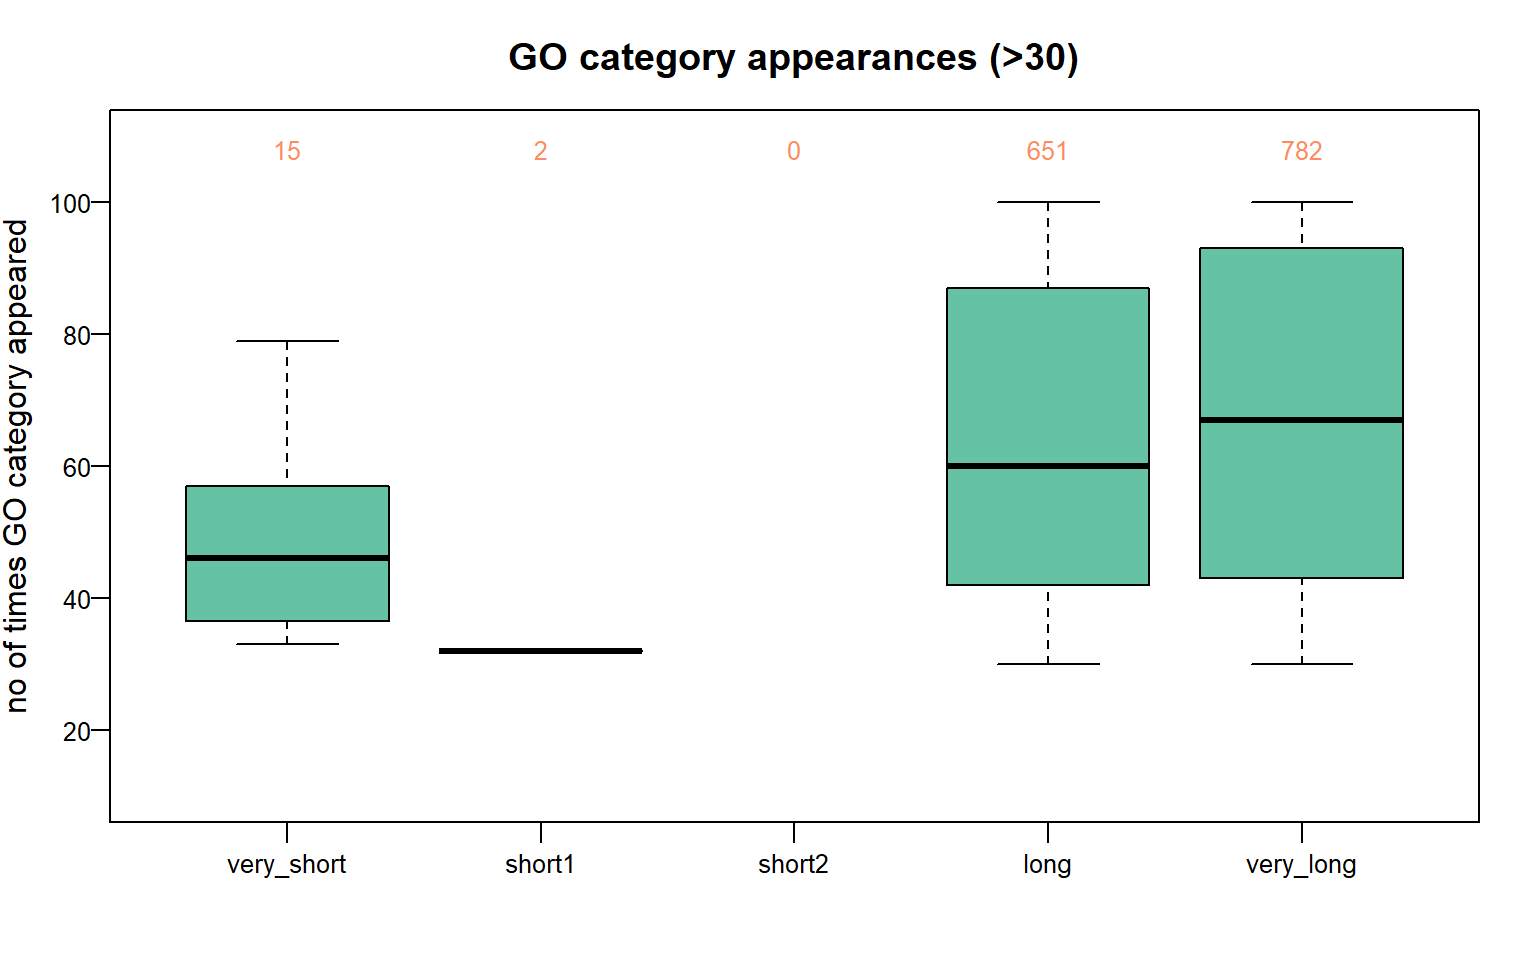
\includegraphics{1.length_biased_files/figure-latex/unnamed-chunk-16-1.pdf}

Replot just showing the data for categories that appeared
\textgreater{}= 10 times

\begin{Shaded}
\begin{Highlighting}[]
\NormalTok{filtered_categories <-}\StringTok{ }\KeywordTok{lapply}\NormalTok{(ordered_categories, }\ControlFlowTok{function}\NormalTok{(x) x[x }\OperatorTok{>=}\StringTok{ }\DecValTok{10}\NormalTok{])}

\KeywordTok{beanplot}\NormalTok{(}
\NormalTok{  filtered_categories, }
  \DataTypeTok{what   =} \KeywordTok{c}\NormalTok{(}\DecValTok{0}\NormalTok{,}\DecValTok{1}\NormalTok{,}\DecValTok{0}\NormalTok{,}\DecValTok{1}\NormalTok{), }
  \DataTypeTok{col    =} \KeywordTok{c}\NormalTok{(}\StringTok{"#1B9E77"}\NormalTok{,}\StringTok{"#06086d"}\NormalTok{), }
  \DataTypeTok{ll     =} \FloatTok{0.03}\NormalTok{, }
  \DataTypeTok{method =} \StringTok{"jitter"}\NormalTok{, }
  \DataTypeTok{border =} \StringTok{"#06086d"}\NormalTok{,}
  \DataTypeTok{las    =} \DecValTok{1}\NormalTok{,}
  \DataTypeTok{log    =} \StringTok{""}\NormalTok{,}
  \DataTypeTok{ylim   =} \KeywordTok{c}\NormalTok{(}\DecValTok{10}\NormalTok{, }\DecValTok{120}\NormalTok{),}
  \DataTypeTok{main   =} \StringTok{"GO category appearances (>10)"}\NormalTok{,}
  \DataTypeTok{ylab   =} \StringTok{"no of times GO category appeared"}
\NormalTok{)}

\KeywordTok{text}\NormalTok{(}\DecValTok{1}\OperatorTok{:}\KeywordTok{length}\NormalTok{(ordered_categories), }
     \DataTypeTok{y   =} \DecValTok{115}\NormalTok{, }
     \DataTypeTok{cex =} \FloatTok{0.8}\NormalTok{, }
     \DataTypeTok{labels =} \KeywordTok{paste0}\NormalTok{(}\StringTok{"n = "}\NormalTok{, }\KeywordTok{sapply}\NormalTok{(filtered_categories, length))}
\NormalTok{     )}
\end{Highlighting}
\end{Shaded}

Now we could do with some stats to pick a cutoff for the number of times
a category appears. Let's just select an arbitrary value of 30 for
now\ldots{}.

Create a dataset that contains these suspect set of categories

\begin{Shaded}
\begin{Highlighting}[]
\NormalTok{suspects <-}\StringTok{ }\KeywordTok{lapply}\NormalTok{(ordered_categories, }\ControlFlowTok{function}\NormalTok{(x) }\KeywordTok{names}\NormalTok{(x[x }\OperatorTok{>=}\StringTok{ }\DecValTok{10}\NormalTok{]))  }

\KeywordTok{sapply}\NormalTok{(suspects, length)}
\end{Highlighting}
\end{Shaded}

\begin{verbatim}
## very_short     short1     short2       long  very_long 
##         48          9          0       1032       1529
\end{verbatim}

\begin{Shaded}
\begin{Highlighting}[]
\NormalTok{print_sums <-}\StringTok{ }\ControlFlowTok{function}\NormalTok{(set1, set2, }\DataTypeTok{not_in =} \OtherTok{FALSE}\NormalTok{) \{}
  \KeywordTok{ifelse}\NormalTok{(}
\NormalTok{    not_in, }
    \KeywordTok{print}\NormalTok{(}\KeywordTok{sum}\NormalTok{(}\OperatorTok{!}\NormalTok{set1 }\OperatorTok\StringTok{ }\NormalTok{set2)), }
    \KeywordTok{print}\NormalTok{(}\KeywordTok{sum}\NormalTok{(set1 }\OperatorTok\StringTok{ }\NormalTok{set2))}
\NormalTok{  )}
\NormalTok{\}}

\KeywordTok{with}\NormalTok{(suspects, \{}
  \KeywordTok{print_sums}\NormalTok{(short1, very_short)}
  \KeywordTok{print_sums}\NormalTok{(short1, very_short, }\OtherTok{TRUE}\NormalTok{)}
  \KeywordTok{print_sums}\NormalTok{(very_short, short2)}
  \KeywordTok{print_sums}\NormalTok{(long, very_long)}
  \KeywordTok{print_sums}\NormalTok{(long, very_long, }\OtherTok{TRUE}\NormalTok{)}
\NormalTok{\})}
\end{Highlighting}
\end{Shaded}

\begin{verbatim}
## [1] 9
## [1] 0
## [1] 0
## [1] 919
## [1] 113
\end{verbatim}

\begin{verbatim}
## [1] 113
\end{verbatim}

All of the categories in the short1 category are found in the very short
category so these can be reduced to one category. The short2 set do not
overlap and can just be renamed to ``short''

The very\_long and long categories have a lot of overlapping categories
so I'll remove any from the long category that are found in the
very\_long category.

\begin{Shaded}
\begin{Highlighting}[]
\NormalTok{suspects}\OperatorTok{$}\NormalTok{long <-}\StringTok{ }\KeywordTok{with}\NormalTok{(suspects, long[}\OperatorTok{!}\NormalTok{long }\OperatorTok\StringTok{ }\NormalTok{very_long])}
\NormalTok{suspects}\OperatorTok{$}\NormalTok{short1 <-}\StringTok{ }\KeywordTok{with}\NormalTok{(suspects, short1[}\OperatorTok{!}\NormalTok{short1 }\OperatorTok\StringTok{ }\NormalTok{very_short])}
\CommentTok{#suspects$short1 <- NULL}
\CommentTok{#names(suspects) <- gsub(names(suspects), pattern = "short2", replacement = "short")}
\KeywordTok{sapply}\NormalTok{(suspects, length)}
\end{Highlighting}
\end{Shaded}

\begin{verbatim}
## very_short     short1     short2       long  very_long 
##         48          0          0        113       1529
\end{verbatim}

\begin{Shaded}
\begin{Highlighting}[]
\NormalTok{suspects <-}\StringTok{ }\NormalTok{suspects[}\KeywordTok{sapply}\NormalTok{(suspects, length) }\OperatorTok{>}\StringTok{ }\DecValTok{0}\NormalTok{]}
\KeywordTok{sapply}\NormalTok{(suspects, length)}
\end{Highlighting}
\end{Shaded}

\begin{verbatim}
## very_short       long  very_long 
##         48        113       1529
\end{verbatim}

\begin{Shaded}
\begin{Highlighting}[]
\CommentTok{#, eval=FALSE\}}
\CommentTok{# write out file with unix line endings}
\ControlFlowTok{for}\NormalTok{ (i }\ControlFlowTok{in} \DecValTok{1}\OperatorTok{:}\KeywordTok{length}\NormalTok{(suspects))\{}
  
  \KeywordTok{ifelse}\NormalTok{(using_laptop,}
\NormalTok{         filename <-}\StringTok{ }\KeywordTok{paste0}\NormalTok{(}\StringTok{"C:/Users/bigginsl/Desktop/temp/biased_gene_lists/identified_categories/"}\NormalTok{, }\KeywordTok{names}\NormalTok{(suspects)[i], }\StringTok{".txt"}\NormalTok{),}
\NormalTok{         filename <-}\StringTok{ }\KeywordTok{paste0}\NormalTok{(}\StringTok{"M:/biased_gene_lists/identified_categories/"}\NormalTok{, }\KeywordTok{names}\NormalTok{(suspects)[i], }\StringTok{".txt"}\NormalTok{)}
\NormalTok{  )}
\NormalTok{  output_file <-}\StringTok{ }\KeywordTok{file}\NormalTok{(filename, }\StringTok{"wb"}\NormalTok{)}
  
  \KeywordTok{write.table}\NormalTok{(}
    \DataTypeTok{file      =}\NormalTok{ output_file,}
    \DataTypeTok{x         =}\NormalTok{ suspects[[i]], }
    \DataTypeTok{row.names =} \OtherTok{FALSE}\NormalTok{,}
    \DataTypeTok{col.names =} \OtherTok{FALSE}\NormalTok{, }
    \DataTypeTok{quote     =} \OtherTok{FALSE}
\NormalTok{  )}
  
  \KeywordTok{close}\NormalTok{(output_file)}
\NormalTok{\}}
\end{Highlighting}
\end{Shaded}


\end{document}
